\documentclass[a4paper, draft]{article}
\pagestyle{headings}


\title{Boltzmann machines and the Hopfield network}

\usepackage{amsmath,amsthm, amsfonts,amscd, amssymb, a4}
\usepackage[final]{graphicx}
\usepackage[final]{listings}
\usepackage{bbm}
\usepackage{empheq}
\usepackage{caption}

\renewcommand\lstlistingname{Algorithm}
\captionsetup[lstlisting]{singlelinecheck=false, margin=0pt, font={sf},labelsep=space,labelfont=bf}




% Theorem environments

%% \theoremstyle{plain} %% This is the default
\newtheoremstyle{own}
    {3pt}                    % Space above
    {3pt}                    % Space below
    {\itshape}                   % Body font
    {}                           % Indent amount
    {\scshape}                   % Theorem head font
    {.}                          % Punctuation after theorem head
    {.5em}                       % Space after theorem head
    {}  % Theorem head spec (can be left empty, meaning ‘normal’)
    
\theoremstyle{own}
\newtheorem{thm}{Theorem}[section]
\newtheorem{cor}[thm]{Corollary}
\newtheorem{lem}[thm]{Lemma}
\newtheorem{prop}[thm]{Proposition}
\newtheorem{ax}{Axiom}[section]

%% \theoremstyle{definition}
\newtheorem{defn}{Definition}[section]

%% \theoremstyle{remark}
\newtheorem{rem}{Remark}[section]
\newtheorem*{notation}{Notation}
\newtheorem{algorithm}{Algorithm}[section]
\theoremstyle{remark}
\newtheorem{example}{Example}[section]

% Fix alignments

% \setlength{\parindent}{0cm}

\newcommand*\widefbox[1]{\fbox{\hspace{4em}#1\hspace{4em}}}
\newcommand*\fullbox[1]{\framebox[\columnwidth]{#1}}

%  Math definitions

% Fields
\newcommand{\R}{\mathbb{R}}
\newcommand{\C}{\mathbb{C}}
\newcommand{\Z}{\mathbb{Z}}
\newcommand{\Q}{\mathbb{Q}}
\newcommand{\N}{\mathbb{N}}
\newcommand{\quat}{\mathbb{H}}

%Groups 
\newcommand{\Lo}{\mathbf{O}(3,1)}
\newcommand{\SL}{\mathbf{SL}}
\newcommand{\SU}{\mathbf{SU}}
\newcommand{\Spin}{\mathbf{Spin}}
\newcommand{\Pin}{\mathbf{Pin}}
\newcommand{\SO}{\mathbf{SO}}
\newcommand{\Poincare}{\mathcal{P}}
\newcommand{\Poincarecov}{\widetilde{\mathcal{P}}}
\newcommand{\Poincareprop}{\widetilde{\mathcal{P}}_+^{\uparrow}}
\newcommand{\Aut}{\mathrm{Aut}}

% Rings
\newcommand{\End}{\mathrm{End}}
\newcommand{\CCl}{\mathbb{C}\mathrm{l}}
\newcommand{\Cl}{\mathrm{Cl}}
\newcommand{\Mat}{\mathrm{Mat}}

% Lie algebras

\newcommand{\spin}{\mathfrak{spin}}
\newcommand{\so}{\mathfrak{so}}
\newcommand{\su}{\mathfrak{su}}
\newcommand{\slc}{\mathfrak{sl}}

%Three-vectors
\newcommand{\xt}{\mathbf{x}}
\newcommand{\yt}{\mathbf{y}}
\newcommand{\pt}{\mathbf{p}}
\newcommand{\nt}{\mathbf{n}}
\newcommand{\sigmat}{\mathbf{\sigma}}

% Vector spaces
\newcommand{\Hil}{\mathcal{H}}

% Other
\newcommand{\calE}{\mathcal{E}}
\newcommand{\calD}{\mathcal{D}}
\newcommand{\calF}{\mathcal{F}}
\newcommand{\calP}{\mathcal{P}}
\newcommand{\Fock}{\mathcal{F}}
\newcommand{\Op}{\mathrm{Op}}

\DeclareMathOperator{\per}{per}
\DeclareMathOperator{\sign}{sgn}
\DeclareMathOperator{\logit}{logit}

\begin{document}
\maketitle




\section{Hopfield networks}

In this section, we will study to start a specific type of neural network called a {\em Hopfield network}, a type of network which has been made popular by J. Hopfield in \cite{Hopfield1982}, even though similar models have been studied by other authors before. In constrast to typical layered networks, in a Hopfield network, each neuron can be connected to any other neuron. This allows excitations to flow through the network, starting at a point and returning to a point - networks with this property are called {\em recurrent} networks.

Still there is a restriction on the weights of a Hopfield network - we assume that the weights are symmetric and no neuron is connected directly to itself, i.e. that
$$
w_{ij} = w_{ji} 
$$
and
$$
w_{ii} = 0
$$
If we let $s_i$ denote the value of neuron $i$, the activation of a neuron is therefore given by
$$
a_i = \sum_{j} w_{ij} s_j = (WS)_i
$$
In this note, we will study binary Hopfield networks, where each neuron can only be in one of two states. Different conventions are in place on how to label these two states, we will use the values $\{ -1, 1\}$. 

So how does the Hopfield network operate? Suppose that the network is in a certain state. i.e. some of the neurons will be "firing", represented by the value $+1$, and others will be passive, represented by the value $-1$. We now choose a neuron at random and calculate its activation function according to the formula above. We then determine the new state by the rule
\begin{align}\label{eq:hopfieldupdaterule}
s_i' = 
\begin{cases} 
+1 & a_i \geq 0 \\
-1 & a_i < 0 
\end{cases}
\end{align}
We now claim that after a finite number of steps, the network has converged, i.e. this rule does not change the state any more. To see this, let us consider the function
$$
E(s) = - \frac{1}{2} \sum_{i,j} w_{ij} s_i s_j
$$
which is called the {\em energy function} of the model. Suppose that we pass from a state $s$ to a state $s'$ by applying the update rule above. Let us assume that we have updated neuron $i$ and changed its state from $s_i$ to $s_i'$. Let 
$$
\Delta s_i = s_i' - s_i
$$
Using the fact that $w$ is symmetric, we can then write
$$
E(s') = -\frac{1}{2} \sum_{p,q \neq i} s_p s_q - \sum_p w_{pi} s_i' s_p
$$
which is the same as
$$
-\frac{1}{2} \sum_{p,q \neq i} s_p s_q - \sum_p w_{pi} s_i s_p
- \sum_p w_{pi} (s_i' - s_i) s_p
$$
Thus we find that
$$
E(s') = E(s) - \Delta s_i \sum_p  w_{ip} s_p
$$
Now the sum is simply the activation of neuron $i$. As our update rule guarantees that the product of $\Delta s_i$ and the activation of $s_i$ is never negative, this implies that during the upgrade process, the energy function will always increase or stay the same. Ignoring the special case that the activation of a neuron is exactly zero\footnote{Some authors modify the update rule to the effect that the state does not change at all if this happens}, we see that we will move into a new state if and only if the energy of the new state is lower than the current energy. Thus the state will settle in a local minimum of the energy function. 

The idea of a Hopfield network is now as follows. In general, there will be more than one local minimum which act as attractors. So regardless of the initial state, the update procedure will eventually converge to the state which is closest to the initial state. This is exactly what we need for an associative memory: the states that the network remembers are local minima of the energy function. If we initialize the network in a state that is already sufficiently close to one of these minima, i.e. if we present the network a distorted version of the memory content, it will converge to the local minimum, i.e. to the original data.

In order to utilize this idea, we need to define a rule that sets the weights according to same state that we want to remember. Thus given some state $s$, we want to construct a weight matrix such that $s$ is a local minimum. More generally, if we have already defined weights giving some local minima, we want to adjust the weights in order to create an additional minimum at $s$, if possible without changing the already existing minima significantly. In \cite{Hopfield1982}, this is done with the following learning rule
\begin{align}\label{eq:hebbrule}
w_{ij} = 
\begin{cases}
\sum_s S^{(s)}_i S^{(s)}_j & i \neq j \\
0 & i = j
\end{cases}
\end{align}
where $S^{(1)}, \dots, S^{(K)}$ are the states that the network should remember. Thus a state $S$ contributes with a positive value to $w_{ij}$ if $S_i$ and $S_j$ have the same sign, i.e. are in the same state. This corresponds to a rule known as {\em Hebbian rule} that has been postulated as a principle of learning by D. Hebb and basically states that during learning, connections between neurons are enforced that fire together (\cite{Hebb}, chapter 4).

Apart from the motivation by a biological analogy, why should this choice of weights be useful? To see this, let us calculate the activation of a neuronal unit if we initialize the weights according to equation \eqref{eq:hebbrule} and the system is in a state $S^{(k)}$.
\begin{align*}
a_i = \sum_{j \neq i} w_{ij} S_j^{(k)} &= 
\sum_{j \neq i} \sum_s S_i^{(s)} S_j^{(s)} S_j^{(k)} \\
&= \sum_{j \neq i} S_i^{(k)} S_j^{(k)} S_j^{(k)} + \sum_{j \neq i} \sum_{s \neq k} S_i^{(s)} S_j^{(s)} S_j^{(k)} \\
&= S_i^{(k)} \sum_{j \neq i}  (S_j^{(k)})^2 + \sum_{s \neq k} S_i^{(s)} 
\sum_{j \neq i} S_j^{(s)} S_j^{(k)} \\
&= S_i^{(k)} (N-1) + \sum_{s \neq k} S_i^{(s)} 
\sum_{j \neq i} S_j^{(s)} S_j^{(k)}
\end{align*}
The first term clearly has the same sign as $S_i^{(k)}$. Now if we assume that the states $S^{(s)}$ are sufficiently uncorrelated, then each of the sums
$$
\sum_{j \neq i} S_j^{(s)} S_j^{(k)}
$$
should be significantly smaller than the number of neurons $N$, as positive and negative terms cancel each other to a large extent. If also the number of patterns that we want to learn is significantly smaller than the number of neurons, then the activation should be dominated by the first term and hence have the same sign as $S_i^{(k)}$. Thus, when we apply the update rule 
\eqref{eq:hopfieldupdaterule} to this state, it will not change. Therefore, if our assumptions are met, the learned states will be stable under the update rule and therefore correspond to points of minimal energy. However, we can only store a limited number of states - as a rule of thumb, only $\approx 0.15 N$ states can be safely stored in a network with $N$ neurons (\cite{Hopfield1982}), otherwise our assumptions break down and the contribution from the terms with $s \neq k$ in the equation above becomes too large to be ignored.

So let us summarize how our model operates. Given a sample $S^{(i)}$ of states to be remembered, we first apply the rule \eqref{eq:hebbrule} to determine the weights. We then accept some distorted input $s$ according to which we initialize states, and then apply the update rule \eqref{eq:hopfieldupdaterule} until the values converge. Then we expect that we arrive at one of the previously stored states, namely the state which resembles the input most.

Let us now think about how we can implement a Hopfield network with $N$ neurons in Python. We can store the state of the network in a column vector with $N$ elements. If we now store all $K$ samples in one matrix $S$ such that each row of the matrix corresponds to one sample, i.e.
$$
S_{ij} = S^{(i)}_j
$$ 
then the learning rule \eqref{eq:hebbrule} turns into
$$
W = S^T S  - K{\mathbbm 1}
$$

Obviously, the update rule can also be expressed as a matrix operation - the sum in \eqref{eq:hopfieldupdaterule} is simply the i-th row of the matrix product of the weight matrix and a state, represented as a column vector. The core part of an implementation of a class {\it HopfieldNetwork} in Python could therefore look as in listing \ref{lst:pythonHopfield}.

\begin{lstlisting}[frame=single,language=Python,caption=Hopfield network in Python, float=ht,label=lst:pythonHopfield]
def learn(self, S):
    #
    # Determine weights based on given sample
    #
    self.W = np.matmul(S.transpose(), S)
    
def update(self):
    #
    # Do a single update
    #
    i = np.random.randint(0,self.N)
    a = np.matmul(self.W[i,:], self.s)
    if a < 0:
        self.s[i] = -1
    else:
        self.s[i] = 1
    
def run(self, state, steps):
    # 
    # Run starting at a given state
    # 
    self.s = state
    for i in range(steps):
        self.update()
    
\end{lstlisting}

Diagram \ref{fig:HopfieldOne} illustrate the output of a small Hopfield network with $N=25$ neurons. In this example, the state of the network is visualized as a 5x5 image, where a black pixel is the value -1 and a white pixel is the value +1. The network has been trained with three patterns, displayed in the first column: one pattern closely resembling a zero, a vertical bar and a horizontal bar. After the training phase, we have then added some noise to the three patterns by randomly flipping 20\% of the neurons into a different state. The second image in each row display the result of that operation. Then the network has been started, and the remaining images in each row display the state after 20, 40, 60 and 80 iterations. We see that the network converges to the saved state after at most 60 iterations. 

\begin{figure}[ht]
\centering
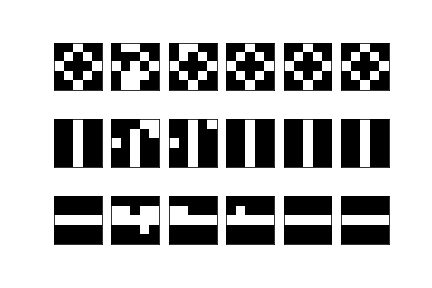
\includegraphics[width=0.7\linewidth]{HopfieldOne}
\caption{Hopfield network with 3 saved states}
\label{fig:HopfieldOne}
\end{figure}


Unfortunately, the network does not always behave that nicely. The next diagram (diagram \ref{fig:HopfieldTwo})) display the results of a simulation with the same network and the same parameters, where we have now changed the initial pattern at 10 randomly chosen points. In addition, we have increased the number of iterations between two subsequent images to 50. Here we see that starting from all the three inital patterns, the network converges, but into a state that is not equal any of the stored target states. Such a state is called a {\em spurios state} and represents an additional local minimum of the energy.

\begin{figure}[ht]
	\centering
	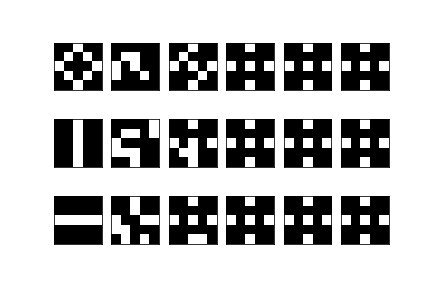
\includegraphics[width=0.7\linewidth]{HopfieldTwo}
	\caption{Hopfield network with spurious stable states}
	\label{fig:HopfieldTwo}
\end{figure}

The situation becomes even worse when we try to store more than three patterns. Diagram \ref{fig:HopfieldThree} shows the results of a trial with five instead of three patterns. This is beyond the limit of $\approx 0.15 N$, i.e. $3.75$ patterns, and in fact we see that the network is not capable to store that amount of information. Even though we have reduced the number of flipped bits to five again and do 50 iterations between any two images, the network does not converge to any of the original states. What actually happens is that the minima that we try to enforce with the Hebbian learning rule merge into one mimimum of the energy that is an attractor for almost all starting states, and the network is no longer able to distinguish between these states.

\begin{figure}[ht]
	\centering
	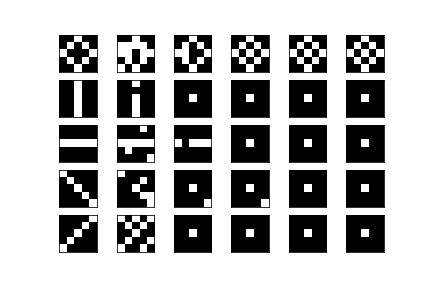
\includegraphics[width=0.7\linewidth]{HopfieldThree}
	\caption{Hopfield network exceeding its capacity}
	\label{fig:HopfieldThree}
\end{figure}

Summarizing, we find that the approach of a Hopfield network to represent patterns as minima of an energy surface works, but the implementation suffers from a few deficiencies: the capacity is low and the network can get trapped in local minima. In the following section, we will study models that are designed to overcome these limitations.


\section{Boltzmann machines}

Let us now return to the realm of neural networks and try to refine the idea of a neural network that implements a Boltzmann distribution at non-zero temperature. More precisely, we consider a neural network consisting of $N$ binary neurons, each of which can have the value $-1$ or $+1$. Every neuron is connected to every other neuron, so that the weights are given by an $N \times N$ matrix that we denote by $W$. We assume that the weight matrix is symmetric, i.e $W^T = W$, and that it is zero along the diagonal, i.e. $W_{ii} = 0$ for all $i$. For a state $x \in \{ -1, 1\}^N$, we define an
energy
$$
E(x) = - \frac{1}{2} \langle x, Wx \rangle = - \frac{1}{2} \sum_{i,j} W_{ij} x_i x_j
$$
We now follow the usual approach to tune our model: we assume that we are given a set of training data ${\mathcal D}$, consisting in $K$ state vectors $s^{(k)}$. Our aim is to adjust the weights of the model in such a way that the Boltzmann distribution 
$$
P(x) = \frac{1}{Z} e^{-\beta E(x)}
$$
models the actual distribution of the training data as closely as possible. It is well known that, if we measure the distance between the "true" distribution and the model distribution using cross-entropy or Kullback-Leibler divergence, finding the best approximation is equivalent to maximizing the likelihood, i.e. the probability that the the observed data originates from independent draws from the model distribution. To do this, let us again calculate the log likelihood function.
\begin{align*}
l({\mathcal D} | W) &= - \frac{1}{K} \ln P({\mathcal D} | W) \\
&= - \frac{1}{K} \sum_k \ln P(x^{(k)} | W) \\
&= - \frac{1}{K} \sum_k \left[ \ln e^{-\beta E(x^{(k)})} - \ln Z \right] \\
&=  \frac{\beta}{K} \sum_k E(x^{(k)}) + \ln Z
\end{align*}


Now, the obvious approach to solving this optimization problem is to apply a gradient descent algorithm to the likelihood function. To do this, we need to calculate the gradient, and we need an efficient way to do this. So let us take the derivatives of the two terms that make up the likelihood function. We start with the second term, which turns out to be an expectation value, namely the expectation value of the derivative of the energy with respect to the model distribution $P$. 
\begin{align*}
\frac{\partial}{\partial W_{ij}} \ln Z &= 
\frac{1}{Z} \frac{\partial}{\partial W_{ij}} Z \\
&= \frac{1}{Z} \sum_x \frac{\partial}{\partial W_{ij}} e^{-\beta E(x)} \\
&= - \beta \frac{1}{Z} \sum_x e^{-\beta E(x)} \frac{\partial}{\partial W_{ij}} E(x) 
= - \beta \langle \frac{\partial}{\partial W_{ij}} E(x) \rangle_P
\end{align*}
Now the partial derivative of the energy is easily calculated. We find that
$$
\frac{\partial}{\partial W_{ij}} E(x) = 
- \frac{1}{2} \frac{\partial}{\partial W_{ij}}  \sum_{p,q} W_{p,q} x_p x_q = 
- \frac{1}{2} x_i x_j
$$ 
and therefore
$$
\frac{\partial}{\partial W_{ij}} \ln Z = \frac{\beta}{2} \langle x_i x_j \rangle_P
$$
The first term is even easier. 
$$
\frac{\partial}{\partial W_{ij}} \frac{\beta}{K} \sum_k E(x^{(k)}) 
= - \frac{\beta}{2} \frac{1}{K} \sum_k  \sum_k  x_i^{(k)} x_j^{(k)}
$$
But this is proportional to an expectation value, namely to the expectation value of $x_i x_j$ under the empirical distribution defined by the data:
$$
\frac{\partial}{\partial W_{ij}} \frac{\beta}{K} \sum_k E(x^{(k)})  = - \frac{\beta}{2} 
\langle x_i x_j \rangle_{\mathcal D}
$$
Thus we have shown that
\begin{align}\label{eq:boltzmannmachinegradient}
\frac{\partial}{\partial W_{ij}} l({\mathcal D} | W) =
- \frac{\beta}{2}  \left[    \langle x_i x_j \rangle_{\mathcal D} - 
\langle x_i x_j \rangle_P       \right]
\end{align}
This formula for the gradient corresponds to the following rule for the weight updates of a Boltzmann machine during the learning phase:
\begin{align}
\label{eq:boltzmannweightupdates}
\Delta W_{ij} = \frac{1}{2} \lambda \beta \left[    \langle x_i x_j \rangle_{\mathcal D} - 
\langle x_i x_j \rangle_P       \right]
\end{align}
where $\lambda$ is the step size chosen for the gradient descent.

Let us pause for a moment and look at this equation. First, it is reassuring to see that this is symmetric in $i$ and $j$, i.e. if we start with a symmetric weight matrix $W$ and update the weights according to the gradient descent algorithm, we will again produce a symmetric matrix. A similar observation holds for the diagonal elements - as $x_i^2 = 1$ for all neurons, both expectation values will be one if $i = j$ and therefore $\Delta W_{ii}= 0$. Thus if $W_{ii}  = 0$ holds before the update it will also hold after the update.

Second, it is instructive to compare this rule to the Hebbian learning rule. The first term is exactly the term that we used for the Hebbian learning rule for a Hopfield network - if two neurons are strongly correlated in the test data set, we strengthen their connection, if the correlation of the neurons is negative we weaken the connection. The second term, however, is new. If we wanted to actually calculate this term, we could use a Gibbs sampler for the full distribution, i.e. we would start at some random point and would allow the network to update itself according to the Gibbs sampling update rule until convergence has been reached. Pushing the analogy with a biological system even further, one could call this process "daydreaming". 

The third interesting observation that we can make is that this learning rule implies that the network cannot distinguish two distribution with the same second moments. In fact, as we have defined it, our network can only learn distributions with a vanishing expectation value for each of the $x_i$, as the Boltzmann distribution is not symmetric (this is not a serious restriction, as we could either add a bias which would produce a non-zero expectation value, or could normalize the data to have expectation zero). If we assume both the data and the model under the distribution $P$ have $\langle x_i \rangle = 0$, the expectation values in \eqref{eq:boltzmannweightupdates} are the elements of the covariance matrix $cov(x_i, x_j)$. Thus the learning stops once the covariance matrix of $P$ has converged to the covariance matrix of the empirical distribution according to the data, and the network is not able to detect any higher moments of the sample distribution. 

Phrased differently (and on purpose a bit less precisely), the network will only be able to learn a distribution that can be reconstructed entirely from its second moments. This does of course restrict the class of distributions that the network is able to learn. To solve this, we can, however, introduce {\em hidden variables}, in a way which is very similar to the hidden units in a layer feed-forward network. Thus we designate certain units of the network as visible units that correspond to input and output of the network, and treat the other units as hidden units which allow the network to represent internal states which are not part of the input or output.

Let us introduce some notation to make this notion precise. We decompose our set of neurons as
$$
\{ 1, \dots, N \} = I_v \cup I_h
$$
and call a neuron $x_i$ hidden unit if $i \in I_h$ and visible unit if $i \in I_v$. We can then write our state space as
$$
\{ -1, 1\}^N = {\mathcal S} = {\mathcal V} \times \mathcal {H}
$$
and write every state as
$$
x = (v,h)
$$
The purpose of the training is now to adjust the weights such that the marginal distribution
$$
P(v) = \sum_h P(v,h) = \frac{1}{Z} \sum_h e^{-\beta E(v,h)}
$$
approximates the empirical distribution of the observed data. As before, we can write down the negative log likelihood function:
\begin{align*}
l({\mathcal D} | W) &= - \frac{1}{K} \ln P({\mathcal D} | W) \\
&= - \frac{1}{K} \sum_k \ln P(v^{(k)} | W) \\
&= - \frac{1}{K} \sum_k  \ln \sum_h e^{-\beta E(v^{(k)},h)}+  \ln Z
\end{align*}

The first term has an interesting interpretation. If we fix the visible units and take the sum of the exponentials of the energies over the hidden units, as we do it here, we obtain something that resembles a partition function conditioned on the visible units. Consequently, the logarithm of this quantity
$$
F(v) = - \ln \sum_h e^{-\beta E(v^{(k)}, h)}
$$
is often called the {\em free energy}. The first term can then be interpreted as the average free energy of the data set.

Now let us see what we know about the gradient of the likelihood function. The derivative of the second term is as before:
$$
\frac{\partial}{\partial W_{ij}} \ln Z = \frac{\beta}{2} \langle x_i x_j \rangle_P
$$
However, we get a more complex expression for the first term. To derive this, let us first calculate
\begin{align*}
\frac{\partial }{\partial W_{ij}} \ln \sum_h e^{-\beta E(v,h)} &= 
\frac{1}{\sum_h e^{-\beta E(v,h)}} \sum_h \frac{\partial }{\partial W_{ij}}
e^{-\beta E(v.h)} \\
&= \frac{1}{Z  P(v)} \sum_h \frac{\partial }{\partial W_{ij}}
e^{-\beta E(v.h)} \\
&= - \beta \frac{1}{Z  P(v)} \sum_h \frac{\partial E(v,h)}{\partial W_{ij}} e^{-\beta E(v,h)} \\
&= - \beta \frac{1}{P(v)} \sum_h \frac{\partial E(v,h)}{\partial W_{ij}} P(v,h) \\
&= - \beta \sum_h \frac{\partial E(v,h)}{\partial W_{ij}} P(h | v)  
= - \beta \langle \frac{\partial E(v,h)}{\partial W_{ij}} \rangle_{P(\cdot | v)}
\end{align*}
So again, an expectation value appears in our calculations, this time it is the expectation value of the partial derivative of the energy with respect to the conditional distribution $P(\cdot | v)$. Thus we find that
\begin{align*}
\frac{\partial }{\partial W_{ij}} l({\mathcal D} | W) &= 
 \beta \frac{1}{K} \sum_k \langle \frac{\partial E(v,h)}{\partial W_{ij}} \rangle_{P(\cdot | v^{(k)})} + \frac{\beta}{2} \langle x_i x_j \rangle_P \\
 &= \frac{\beta}{2} \left[
 - \langle \langle  x_i x_j \rangle_{P(\cdot | v)} \rangle_{\mathcal D}
 + \langle x_i x_j \rangle_P  \right]
\end{align*}
and obtain the update rule
\begin{align}\label{eq:boltzmannhiddenupdaterule}
\Delta W_{ij} = \frac{1}{2} \lambda \beta \left[
 \langle \langle  x_i x_j \rangle_{P(\cdot | v)} \rangle_{\mathcal D} 
 - 
 \langle x_i x_j \rangle_P  
 \right] 
\end{align}
Note that the first term is a double expectation value. For every $v$ in the test data set, we form the expectation value over all values of $x_i x_j$, where the visible units are set to $v$, under the distribution $P(\cdot | v)$, and then we average this over the entire test data set.

With this update rule, we could now theoretically obtain the gradient as follows. For each input $v$ in the test data, we first clamp the visible units to $v$. We then run a Gibbs sampler across the hidden units to calculate the first expectation value (it is straightforward to see that running a Gibbs sampler while keeping the visible units fixed is the same as running a Gibbs sampler for the conditional distribution). We repeat this procedure for each input vector and add up the results. This phase is called the {\em positive phase}. 

Then we release the visible units and run a Gibbs sampler for the full distribution. We sample the expectation value of $x_i x_j$ from this Markov chain and subtract the result from the previously computed value. This phase is called the {\em negative phase}. Finally, we multiply by the step size and the inverse temperate and add the result to $W_{ij}$. 


Using Markov chains to obtain a gradient in this way works, but obviously requires a lot of computational steps. To calculate one gradient, we have to run two Markov chains to converge - and we have seen in our simulations of the Ising model that even for a comparatively small system with a comparatively simple weight matrix, this can easily required a few million iterations -  and we have to repeat this procedure for every iteration of the gradient descent! Thus this algorithm is hardly useful.

So it looks like we have reached a dead end - we have found a way to apply gradient descent to a Boltzmann machine, but found that the computational complexity is intractable. Fortunately, it turns out that this changes substantially if we impose a restriction on our model - we require that there are no connections between the individual units and no connections between the hidden units. This model is called a {\em restricted Boltzmann machine}. We can think of this as a layered model, with a layer of hidden units and a layer of visible units, where only connections between layers are allowed, as illustrated in diagram \ref{fig:RestrictedBoltzmannMachine}. This model seems to be restricted, but is actually still very powerful and in some sense universal. It can in fact be shown (\cite{BengioRoux2007} that every binary distribution can be approximated arbitrarily well by a restricted Boltzmann machine if we only allow sufficiently many hidden units. 


\begin{figure}[ht]
\centering
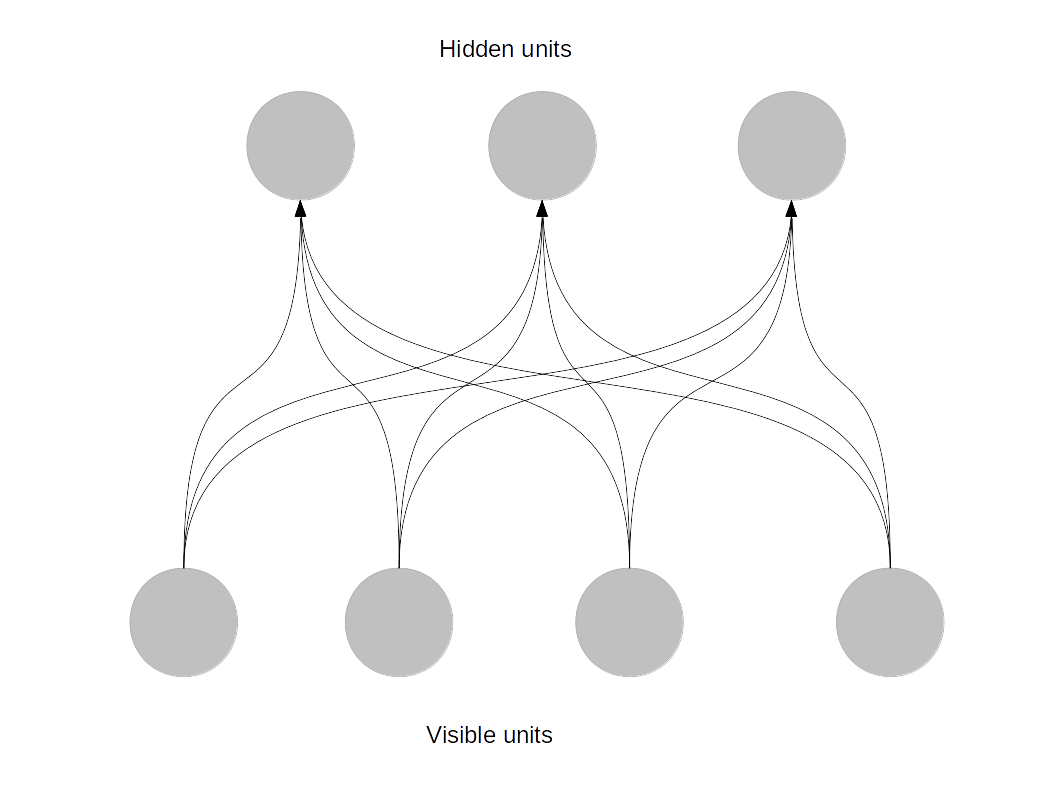
\includegraphics[width=0.9\linewidth]{RestrictedBoltzmannMachine}
\caption{Restricted Boltzmann machine}
\label{fig:RestrictedBoltzmannMachine}
\end{figure}

Different from our previous conventions, we will now use $\{ 0,1 \}$ instead of $\{ -1, 1\}$ as the values of the neurons. When we again denote the index set for the visible units by $I_v$ and the index set for the hidden units by $I_h$, we can write the energy of this model as
$$
E(v,h) = - \sum_{i \in I_v, j \in I_h} W_{ij} v_i h_j - \sum_i v_i b_i - \sum_j h_j c_j
$$
where the $b_i$ and $c_j$ represent a bias for the visible respective hidden units.
Of course the matrix $W$ is now no longer symmetric, as it is already the reduced matrix of connections. Instead, $W$ is a matrix with $m$ rows and $n$ columns, where $m$ is the number of visible units and $n$ is the number of hidden units.

So far, we have not yet worked with a bias, so we need to derive the update rules for the bias first. The calculation is more or less the same as for the weights - the gradient is given by a difference of expectation values of the derivative of the energy. Of course
$$
\frac{\partial E}{\partial b_i} = - v_i
$$
and
$$
\frac{\partial E}{\partial c_j} = - h_j
$$
so that the update rules for the bias are
$$
\Delta b_i = \lambda \beta \left[
\langle \langle  v_i \rangle_{P(\cdot | v)} \rangle_{\mathcal D} 
- 
\langle v_i \rangle_P  
\right] 
$$
and
$$
\Delta c_j = \lambda \beta \left[
\langle \langle  h_j \rangle_{P(\cdot | v)} \rangle_{\mathcal D} 
- 
\langle h_j \rangle_P  
\right] 
$$

Let us now turn again to the update rule for the weights.
The derivatives of the energy with respect to $W_{ij}$ are now
$$
\frac{\partial E}{\partial W_{ij}} = - v_i h_j
$$
and the update rule for the weights turns into
$$
\Delta W_{ij} = \\
 \lambda \beta \left[
\langle \langle  v_i h_j \rangle_{P(\cdot | v)} \rangle_{\mathcal D} 
- 
\langle v_i h_j \rangle_P  
\right] 
$$
Now let us start to simplify this expression a bit further, leveraging the restrictions on the geometry of the network. Let us first try to find an expression for the conditional probability
$$
P(h_j = 1 | v)
$$
This is in fact easy to calculate in our situation. As the state of a hidden unit does not depend on the other hidden units, but only on the visible unit, we find that
$$
P(h_j = 1 | v)=  \sigma(\beta (\sum_i W_{ij} v_i + c_j)) 
$$
Using this, we can already simplify the first term in the update rule as follows:
\begin{align*}
\langle v_i h_j \rangle_{P(\cdot | v)} &= \sum_h P(h | v) v_i h_j \\
&= v_i   \sum_{h : h_j = 1} P(h | v)   \\
&= v_i P(h_j = 1 | v) = v_i \sigma(\beta (\sum_i W_{ij} v_i + c_j)) 
= v_i \sigma(\beta (W^T v)_j + c_j)
\end{align*}
This is good news - we do not need to sample from the model distribution to calculate this! So let us see whether a similar simplification works for the second term.  In fact, the second term can be written as an expectation value over the marginal distribution:
\begin{align*}
\langle v_i h_j \rangle_P &= \sum_v \sum_h v_i h_j P(v,h) \\
&= \sum_v v_i P(v) \sum_h h_j P(h | v) \\
&= \sum_v v_i \sigma(\beta W^T v) P(v) = \langle v_i \sigma(\beta ((W^T v)_j + c_j)) \rangle_{P(v)}
\end{align*}
so that we now arrive at the update rule
\begin{align}\label{eq:rbmupdaterule}
\Delta W_{ij} = \beta \left[
\langle v_i \sigma(\beta (W^T v)_j + c_j) \rangle_{\mathcal D}
-
\langle v_i \sigma(\beta (W^T v)_j + c_j) \rangle_{P(v)}
\right]
\end{align}
Thus again, we see that the gradient is composed of two terms, which we again call the {\em positive phase} and the {\em negative phase}. In each phase, we sample the same expression, once over the data distribution and once over the marginal distribution.

Whereas we have found an analytic expression for the positive phase, there is no obvious analytic expression for the negative phase, so we again need a sampling procedure to calculate this term. At this point, the special structure of the network again helps to make the sampling easier. Suppose we wanted to apply an ordinary Gibbs sampler, where instead of choosing the neuron that we update next randomly, we cycle sequentially through all the neurons. We could then do all the hidden neurons first and then continue with the visible units. Now, as the visible units only depend on the hidden units and vice versa, we could as well update all hidden units in parallel and then all visible units in parallel, using that as in the case of hidden units, the conditional probability for a visible unit to be one can be expressed as
$$
P(v_i = 1 | h) = \sigma(\beta (\sum_j W_{ij} h_j + b_i))
$$ 
This procedure is called {\em Gibbs sampling with block updates}. It is also obvious that sampling from the joint distribution $P(v,h)$ in this way and then ignoring the values of the hidden units in this way gives a sampler for the marginal distribution. 

Therefore our algorithm to calculate the second term of the update rule would be as follows. We would start with some value for the visible units. Then we would calculate the probability that each hidden unit is on given these values for the visible units and update the hidden units according to this distribution. We would then use the new values for the hidden units, calculate the conditional distribution of the visible units and update the visible units according to this distribution. This would constitute a full Gibbs sampling step. We would repeat this process until convergence is reached and then sample for a few steps to calculate the expectation values above. Plugging this into the update rule \eqref{eq:rbmupdaterule} and calculating the first term analytically, we would then obtain the needed update for the weights.

This sampling approach still requires to run a Markov chain until convergence, so we have not yet solved the problem of the high computational complexity. Now it turns out that several approaches exist to reduce the computational effort by replacing the gradient by an approximation. One approach which has become very popular is called {\em contrastive divergence} and was introduced in \cite{Hinton2002} (see also \cite{FischerIgel2014} for a review and summary). 

The first approximation that the contrastive divergence algorithm makes is to replace the expectation value over the marginal distribution by a point estimate. So we run a Markov chain for a given number of steps, say $k$, and then use the value
$$
v_i \sigma(\beta ((W^T v)_j + c_j))
$$
at the final location of the chain as an approximation for the expectation value. The idea behind this is that, as we repeat this procedure anyway for each step of the gradient descent and the distribution only changes slightly between any two subsequent steps, the outer loop of the gradient descent will already provide an averaging so that a point estimate should give a good first approximation.

The second simplification behind the algorithm is that we start the sample not at an arbitrary, randomly chosen value for the visible units, but at one of the data points. We then sample only a very small number $k$ of steps. Somehow surprisingly, it turns out that even $k=1$, i.e. one full Gibbs sampling step, suffices in practice to obtain a reasonable approximation! 

We can apply the same procedure to the bias and obtain an algorithm which is called {\em one-step contrastive divergence} or {\em CD-1} and is spelled out in algorithm \ref{lst:cdone}. 



\begin{lstlisting}[mathescape=true,frame=single, label=lst:cdone, float=ht,
captionpos=t, caption=One-step contrastive divergence]
For each iteration do
  Sample a vector $v$ from the data set
  Set $e = \sigma(\beta( W^T v + c))$
  For each hidden unit
  set $h_j = 1$ with probability $e_j$
  For each visible unit
  set $\bar{v}_i = 1$ with probability $\sigma(\beta (W h + b))_i$
  Set $\bar{e} = \sigma(\beta (W^T \bar{v} + c))$
  Set $W = W + \lambda \beta \left[  v e^T - \bar{v} \bar{e}^T  \right]$
  Set $b = b + \lambda \beta \left[  v - \bar{v}  \right]$
  Set $c = c + \lambda \beta \left[  e - \bar{e}  \right]$
Done
\end{lstlisting}


It is far from obvious why this algorithm gives useful results. Usually, we would expect that reducing a full Markov chain to a single step would yield the result essentially useless. In fact, it is known that in some cases, CD-1 converges slowly or not at all or does not converge to the gradient of the log likelihood so that other algorithms like persistent contrastive divergence are required (see \cite{FischerIgel2014} for a summary of some theoretical results and further references). 

In any case, the algorithm is intuitively very appealing. We feed a sample from the training data set into the visible units, then forward the signal to the hidden units and sample from the hidden units to obtain a {\em reconstruction} of the training data. The weight update is then driven by the difference in the correlations between the original data and the hidden units and the reconstruction and the corresponding activations of the hidden units. 


Even though constrastive divergence is very popular, alternative approaches to training restricted Boltzmann machines exist. We will look at one example in detail. 

Remember that the key idea of the contrastive divergence algorithm is to start the Gibbs sampling procedure that is needed to calculate the contribution of the negative phase at a point which is hopefully close to the equilibrium state, namely a sample from the data set. For each iteration, a different sample is chosen, and therefore the chain is restarted with every iteration. The idea behind an algorithm known as {\em persistent contrastive divergence (PCD)} (see \cite{Tieleman2008}) is to instead of a data point the result of the previous iteration as starting point for a Gibbs sampling step. Thus in every iteration, we perform one Gibbs sampling step, save the result and use it as the starting point of the Gibbs sampling step for the next iteration.

Effectively, this amounts to running a long chain of states related by Gibbs sampling steps. In practice, more than one chain is used. Such a chain is often called a {\em negative particle}. Note that this is not a Markov chain, as we adapt the model parameters during each iteration and therefore the Markov kernel changes in each step. However, the idea is that if we use small step sizes, the resulting chain will be almost a Markov chain, as the model parameters only change slightly. Therefore we should expect that this approach works best with a small step size. Unfortunately, this slows down convergence, so that it is common to reduce the step size after each iteration.

We close these notes with a slightly different interpretation of Boltzmann machines. The energy of a restricted Boltzmann machine has the interesting property that the energy of a state, specified by the values of the visible and hidden units, can be written as a sum of terms each of which involves the value of only one hidden unit. Specifically, we can write
\begin{align*}
E(v,h) &= - \sum_{ij,j} W_{ij} v_i h_j - \sum_i v_i b_i - \sum_j h_j c_j \\
&= - \sum_i v_i b_i - \sum_j h_j \left[ \sum_i W_{ij} v_i + c_j \right] \\
&= - \langle v,b \rangle - \sum_j h_j a_j
\end{align*}
where $a_j$ is the activation of the hidden unit $j$, which depends only on the values of the visible units and the parameters of the model. Thus we can write
$$
E(v,h) = f(v) + \sum_j g_j(h_j)
$$
with functions $f$ and $g_j$ parametrized by the weights and biases. Using this, we can now turn the sum of the exponentials of the energy into a product:
\begin{align*}
\sum_h e^{-\beta E(v,h)} &= \sum_{h_1} \sum_{h_2} \dots \sum_{h_n} e^{-\beta E(v,h)} \\&= \sum_{h_1} \sum_{h_2} \dots \sum_{h_n} e^{-\beta f(v) - \beta \sum_j g_j(h_j)} \\
&= e^{-\beta f(v)} \sum_{h_1} \sum_{h_2} \dots \sum_{h_n} \prod_j e^{-\beta  g_j(h_j)} \\
&= e^{-\beta f(v)} \sum_{h_1} e^{-\beta  g_1(h_1)} \sum_{h_2} 
\dots \sum_{h_n} e^{-\beta  g_n(h_n)} \\
&= e^{-\beta f(v)} \prod_j \sum_{h_j} e^{-\beta  g_j(h_j)}
\end{align*}
For a restricted Boltzmann machine, this expression becomes particularly simple as in the sum over the values of each $h_i$, the term for $h_i = 0$ always gives one. We obtain
\begin{align}\label{eq:energyfactorization}
\sum_h e^{-\beta E(v,h)} = e^{\beta \langle v,b \rangle}
\prod_j (1 + e^{\beta a_j})
\end{align}
This allows us to decompose the probability for a given visible unit as product
$$
P(v) = \frac{e^{\beta \langle v,b \rangle}}{Z} \prod_j (1 + e^{\beta a_j})
$$
which shows that a restricted Boltzmann machine is an instance of a larger class of models called {\em product of experts}. Here, each hidden unit takes the role of an expert that provided a probability depending on the input of that hidden unit only, i.e. on what the expert can "see". The probabilities returned by the individual experts are then multiplied and normalized to obtain an overall probability. We also remark that equation \ref{eq:energyfactorization} can be used to effectively calculate the free energy, as it implies that
$$
F(v) = - \beta \langle v, b \rangle - \sum_j \ln (1 + e^{\beta a_j})
$$



%%%%%%%%%%%%%%%%%%%%%%%%%%%%%%%%%%%%%%%%%%%%%%
%% Bibliography
%%%%%%%%%%%%%%%%%%%%%%%%%%%%%%%%%%%%%%%%%%%%%%

\begin{thebibliography}{9}
	

\bibitem{Bishop}
C.M.~Bishop, 
{\em Pattern recognition and machine learning},
Springer, New York 2006

\bibitem{Hopfield1982}
J.J.~Hopfield,
{\em Neural networks and physical systems with emergent collective computational
	abilities},
Proc. Nat. Acad. Sci. Vol. 79, No. 8 (1982), pp. 2554--2558

\bibitem{Hebb}
D.O.~Hebb,
{\em The organization of behaviour},
Wiley, New York 1949

\bibitem{Bengio2009}
Y.~Bengio,
{\em Learning deep architectures for AI},
Foundations and Trends in Machine Learning Vol. 2, No. 1 (2009), 1--127

\bibitem{MacKay}
D.~MacKay,
{\em Information Theory, Inference and Learning Algorithms},
Cambridge University Press, Cambridge 2003

\bibitem{Ising1924}
E.~Ising,
{\em Beitrag zur Theorie des Ferromagnetismus},
Zeitschrift f. Physik, Vol. 31, No.1 (1924), 253--258

\bibitem{Hinton2002}
G.~Hinton,
{\em Training products of experts by minimizing contrastive divergence},
Journal Neural Computation Vol. 14, No. 8 (2002), 1771--1800

\bibitem{FischerIgel2014}
A.~Fischer, C.~Igel,
{\em Training restricted Boltzmann machines: an introduction},
Pattern Recognition Vol. 47 (2014), pp 25--39

\bibitem{Hinton2010}
G.~Hinton,
{\em A practical guide to training restricted Boltzmann machines},
Technical Report University of Montreal TR-2010-003

\bibitem{BengioRoux2007}
N.~Le Roux, Y.~Bengio,
{\em Representational Power of Restriced Boltzmann machines and Deep Belief Networks},
Journal Neural Computation Vol. 20 No. 6 (2008), 1631--1649

\bibitem{Tieleman2008}
T.~Tieleman, 
{\em Training restricted Boltzmann machines using approximations to the likelihood gradient},
International Conference on Machine Learning (ICML) 2008

\bibitem{Swersky2010}
K.~Swersky, B.~Chen, B.~Marlin, N.~de Freitas,
{\em A tutorial on stochastic approximation algorithms for training restricted Boltzmann machines and Deep Belief Nets},
Information Theory and Applications (ITA) Workshop 2010


\end{thebibliography}
\end{document}


